\documentclass[conference]{IEEEtran}
\IEEEoverridecommandlockouts

\usepackage{cite}
\usepackage[hidelinks]{hyperref}
\usepackage{svg}

\def\BibTeX
{
    \rm B\kern-.05em{\sc i\kern-.025em b}\kern-.08em
    T\kern-.1667em\lower.7ex\hbox{E}\kern-.125emX
}

\begin{document}

\title
{
    A Comparative Analysis of Botball Servo Models\\
}

\author
{
    Nico Stolz*, Lukas Sanz, Sebastian Lampl,\\
    Raphael Wiedemann, Johannes Kosche, Stefan Bleier\\
    Höhere Technische Bundes Lehr- und Versuchsanstalt Wiener Neustadt\\
    (Federal Technical Secondary College)\\
    Department of Computer Science\\
    2700 Wiener Neustadt, Austria\\
    **Corresponding author's email: stolz.nico@student.htlwrn.ac.at\\
}

\maketitle
\begin{abstract}
    In this paper, the Botball servos and two possible alternatives have been presented to ensure that OPEN contestants can choose the perfect servo for their specific requirements. Looking at the different designs, it is clear that certain tasks can be better solved with a different model. An example of this is the weight of the servo, which should be as low as possible for a fast and agile robot.

    The four different servos are compared on the basis of various criteria such as price, size, weight, speed and lifting force, all of which are important when choosing a servo.

    At the end there is a clear overview of the data of the servos used in this test. It is recommended to go to \cite{b2} if the servos found here are not sufficient for personal use. By checking the data in each category, it should be easy to find the best servo for any application.

\end{abstract}

\section{Introduction}
    The focus is on identifying the most suitable servo for specific tasks, such as heavy lifting. This paper compares the Absima S90MH and the MEX 85MG servos, along with their standard and micro variants, in the context of Botball robotics. The Absima S90MH and MEX85MG were selected due to limited availability from nearby sellers. These servos are being compared in terms of price, size, weight, speed, and lifting force, which are significant factors when choosing a servo for a specific need. The objective of this work is to inform Botball teams about the specific strengths of the servos they are using, while also providing OPEN teams with possible servo alternatives.

\section {Literature Review}
    The cited work \cite{b1} offers a fundamental insight into servos, making it particularly useful for newcomers to the field. While the study focuses on the comparative analysis of specific servo models, it also explains more general distinctions, such as the difference between standard hobby servos and continuous rotation servos, or the distinction between micro, standard and giant servos. Additionally, it provides a comprehensive understanding of servo mechanics and their operating principles.

    For those OPEN tournament competitors whose requirements extend beyond the four servos analysed in this study, the extensive servo database presented in \cite{b2} is a valuable resource. The servos used for comparison in this paper are not included in this database. Despite the potentially overwhelming array of choices, this database serves as a recommended starting point for identifying the most suitable servo for specific applications.
    
\section {Experimental Setup}
    \subsection{Price}
        The prices were obtained from the official websites cited in references \cite{b3, b4, b5, b6}. To ensure precision, the prices of the Botball servos were converted to EUR and the prices of the possible alternatives were converted to USD. Both prices are presented later in this work. The exchange rate on February 27\textsuperscript{th} was 1.00 USD to 1.09 EUR, as shown in reference \cite{b7}.

    \subsection{Size}
        To ensure precise measurements, the size of each servo was measured using a caliper and split into length, width, and height. While some sources include the servo head and handles in their measurements, others do not. In this paper, the servo head and handles were included in the measurement.
        
    \subsection{Weight}
        Due to the limited availability of specialised measuring instruments, the weight measurements of the servos were conducted using a commercially available scale with a specified accuracy of up to grams. It is important to note that the servo cable was included in the weight, resulting in a small bias in the measurement.
        
    \subsection{Speed}
        The turning servos were recorded on a 60fps camera and analyzed frame by frame. The number of frames required for each servo to turn 60° were counted and used to calculate a value in sec/60° for each servo. The test was repeated 6 times and the arithmetic mean was calculated to ensure accuracy. It is important to note that there is a possibility of bias and the values may be slightly higher or lower.

    \subsection{Lifting Force}
        Servo lifting capacity is typically measured in kg/cm, but precise measurement is difficult. For this work, weight was added incrementally to the servo until it began to struggle. The Botball servos had been in use for an extended period, which may have negatively impacted the data.
    
\section{Results}
    \subsection{Price}
        Price is a crucial factor when selecting a servo. Upon closer inspection of the price data shown in Figure 1, it becomes clear that the Absima S90MH servo is more expensive than the standard Botball servo. Similarly, a comparison between the micro Botball servo and the MEX 85MG shows a similar trend, although with a smaller price difference. When choosing a servo, it is important to carefully consider both the cost and its potential benefits for the robot's design and operation.

        \begin{figure}[htbp]
            \centering
            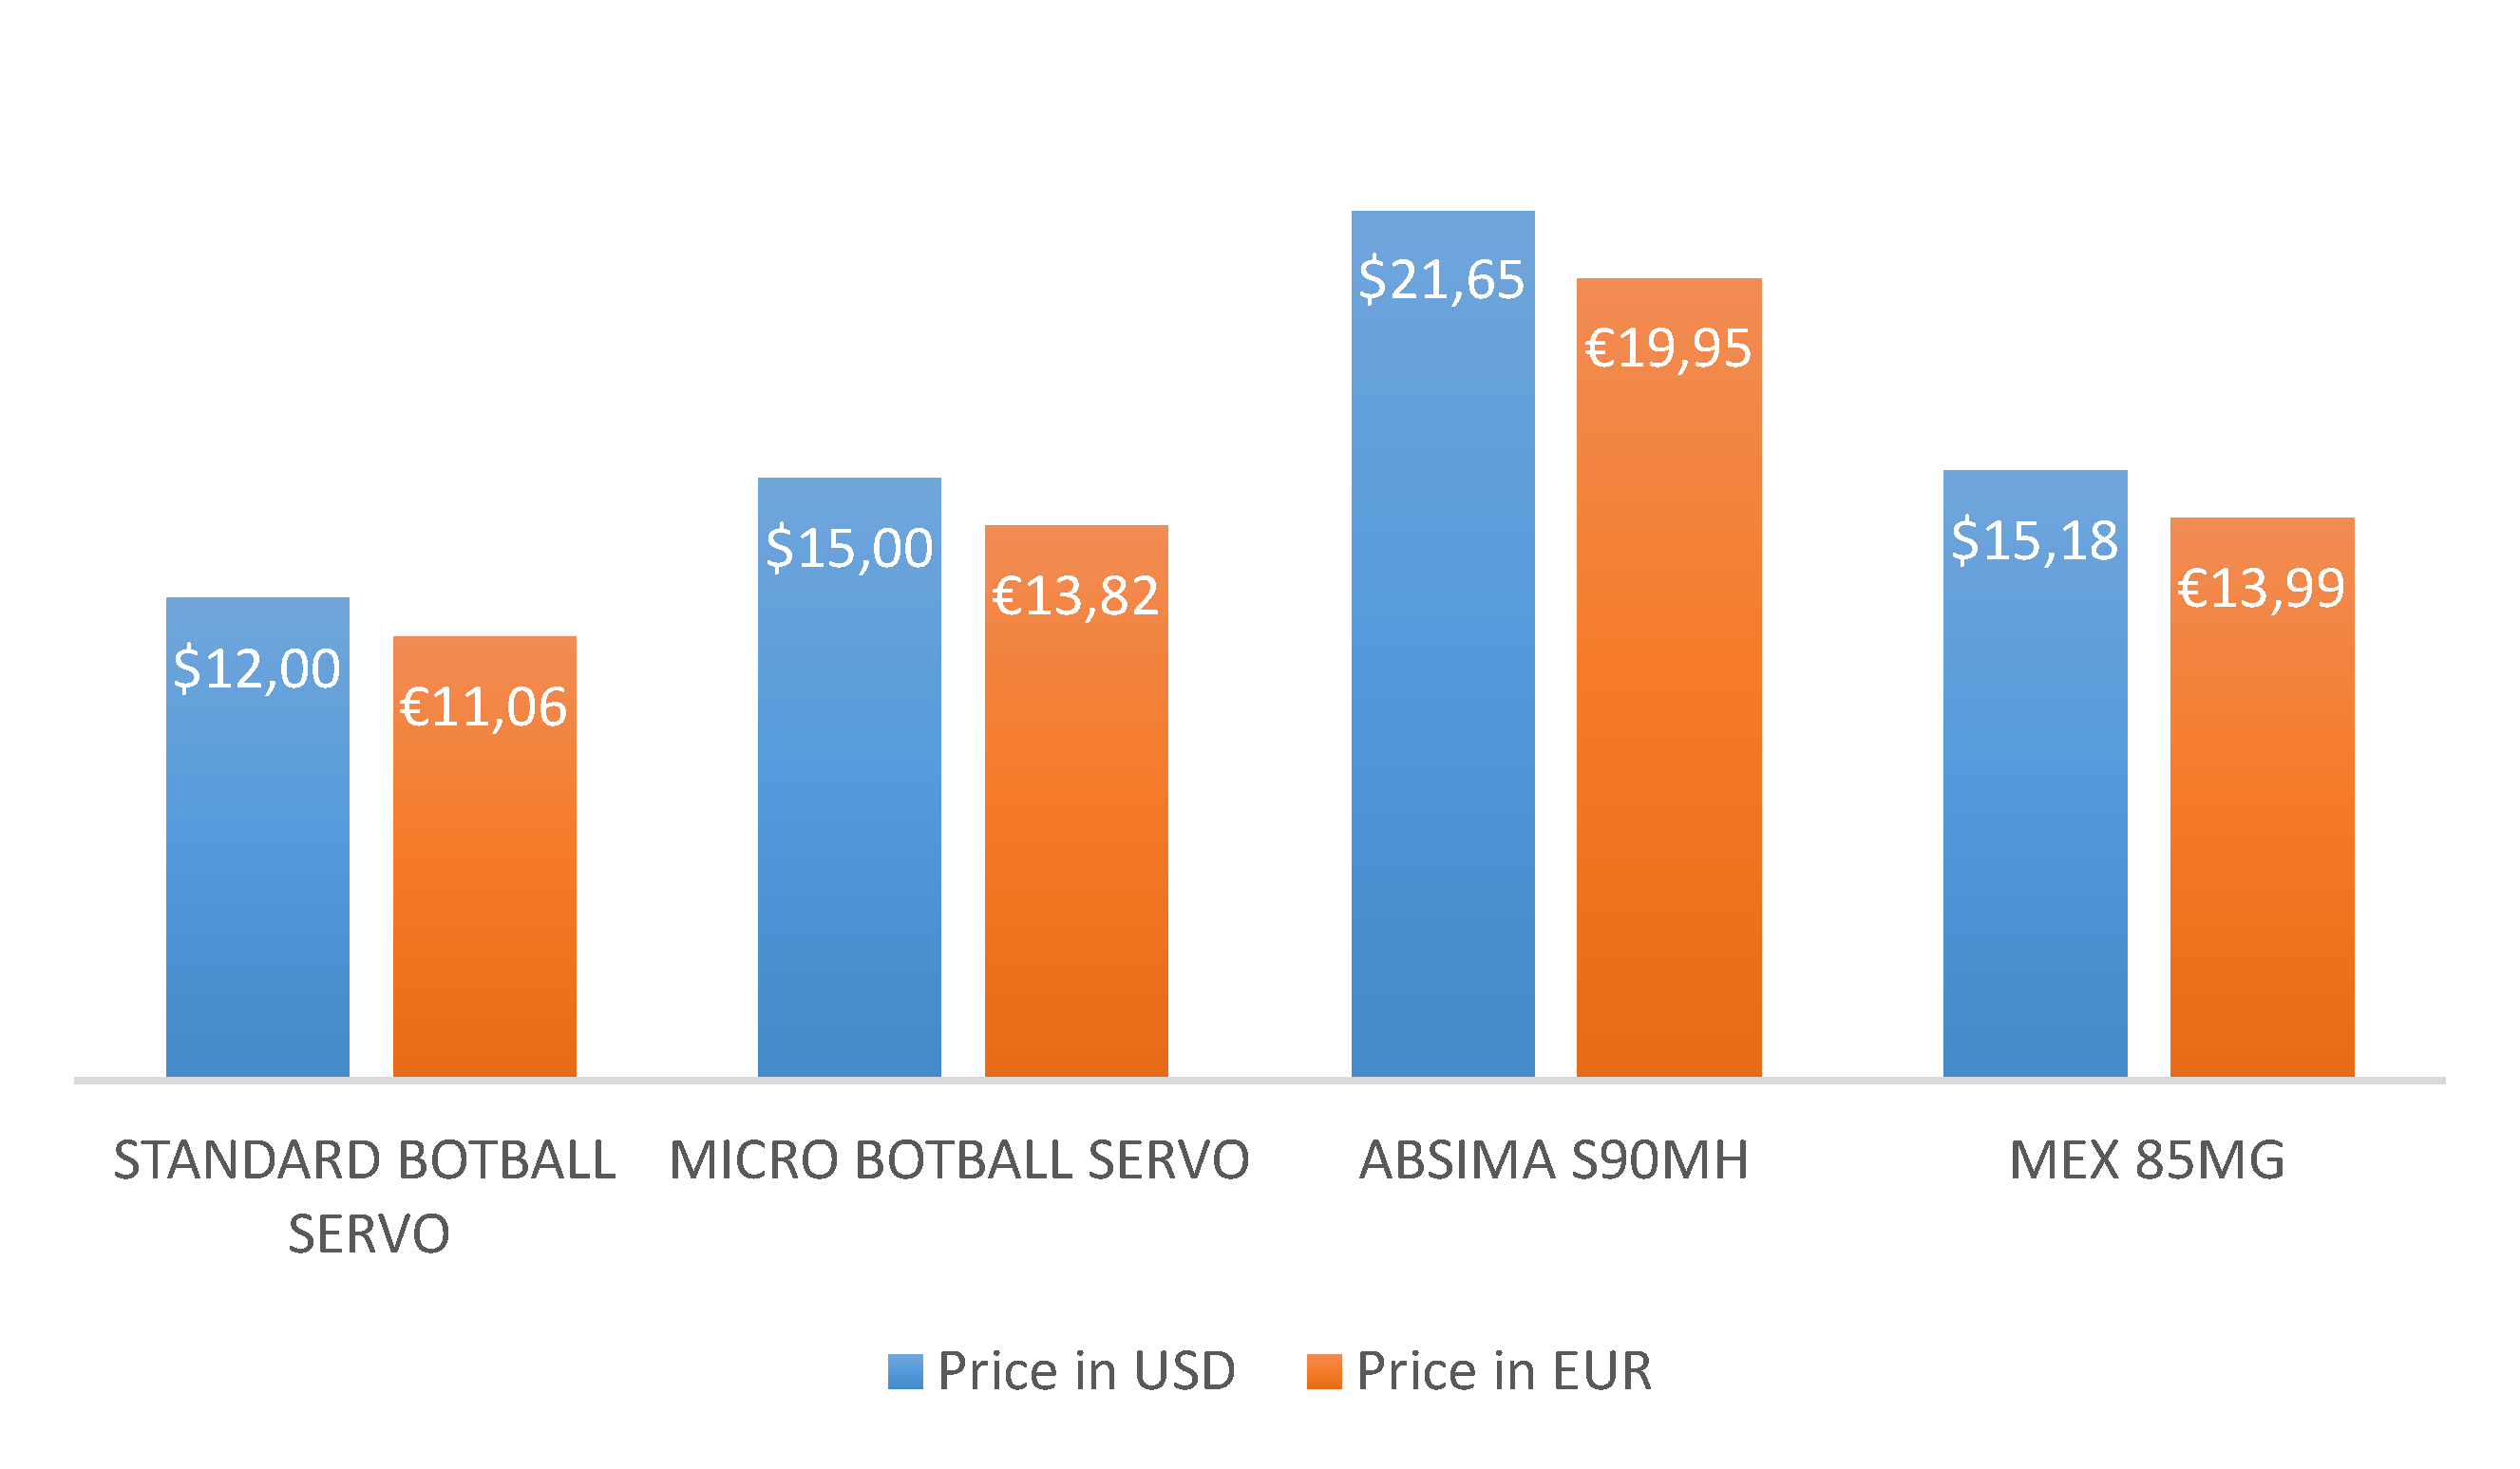
\includegraphics[width=0.50\textwidth,keepaspectratio]{price_chart.pdf}
            \caption{Comparison of servo prices in EUR and USD}
        \end{figure}

    \subsection{Size}
        Servo dimensions are a crucial aspect of robot design, especially in situations with spatial constraints or specific enclosure requirements. Oversized servos can complicate the design process, while smaller ones may offer greater flexibility. Therefore, selecting the appropriate size is essential for optimizing robot functionality.
        
        \begin{figure}[htbp]
            \centering
            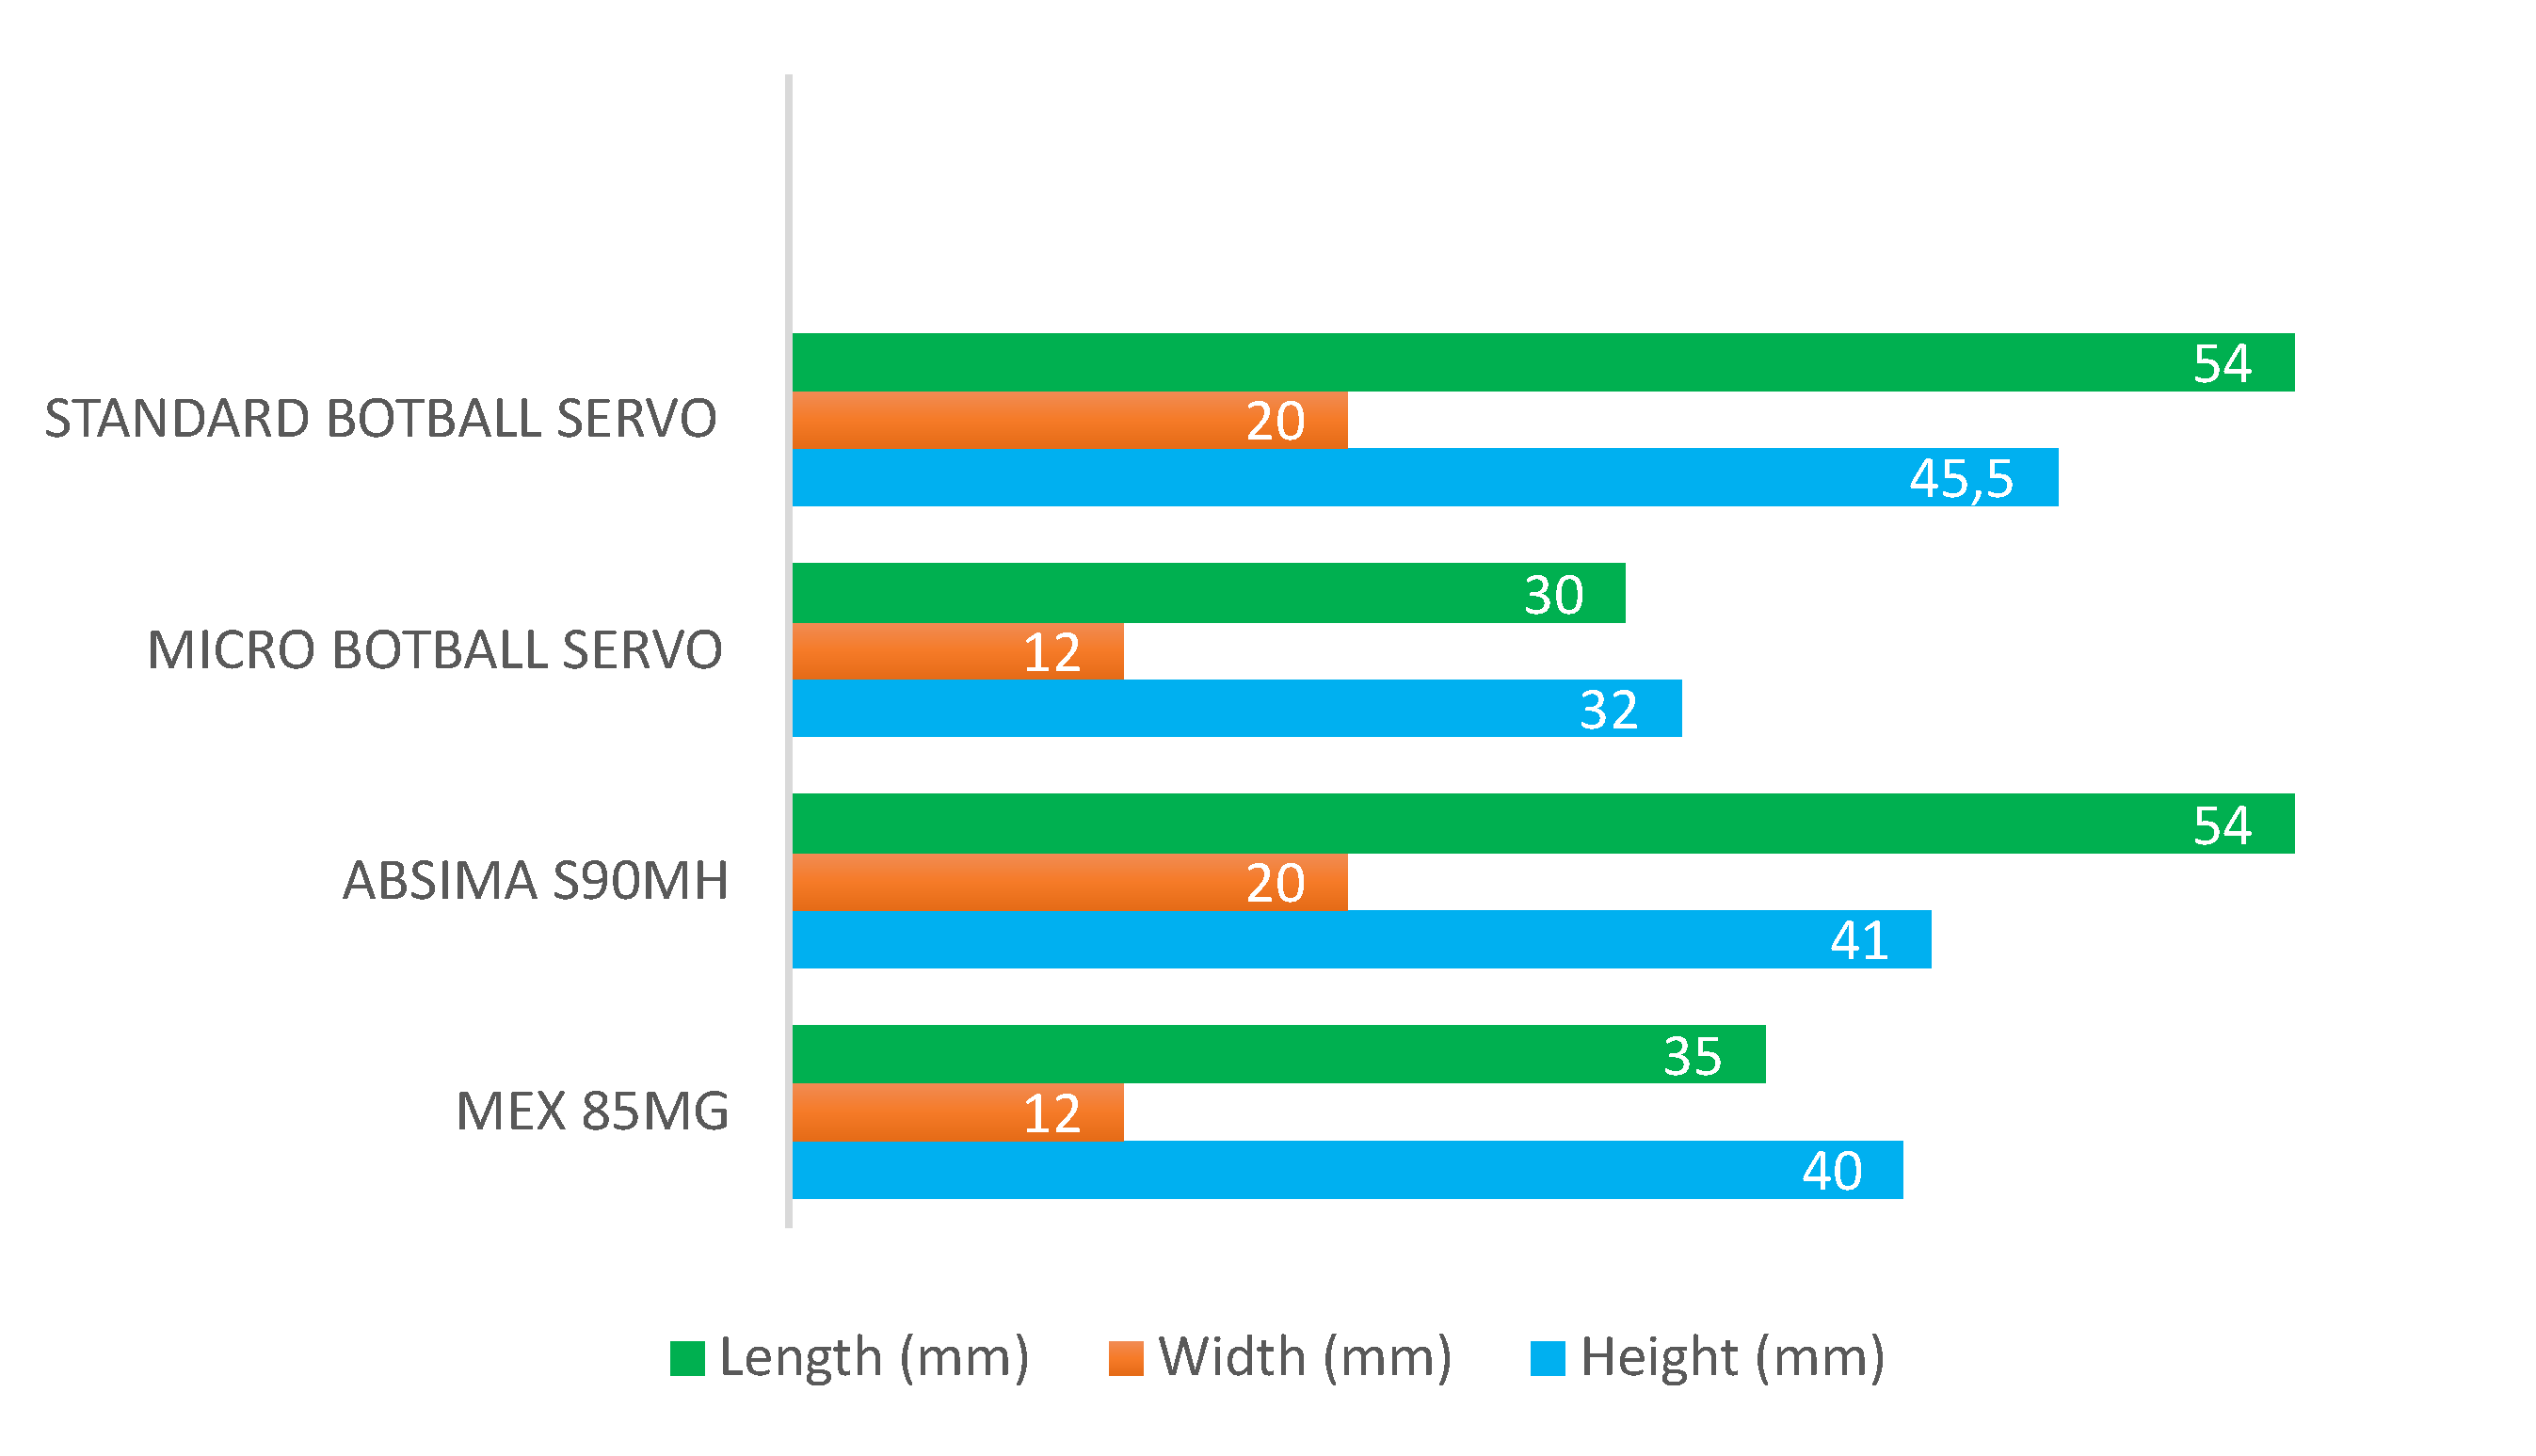
\includegraphics[width=0.50\textwidth,keepaspectratio]{dimensions_chart.pdf}
            \caption{Comparison of servo dimensions in millimeters}
        \end{figure}

        The data shows that the standard Botball servo is larger than the Absima S90MH, while the micro Botball servo is more compact than the MEX 85MG. For OPEN tournament participants who aim to build a smaller robot, the micro Botball servo is the optimal choice. This size comparison, illustrated in Fig. 2, helps designers make informed decisions to meet specific spatial requirements in their robotics projects.

    \subsection{Weight}
        Weight is a crucial factor in robot design and functionality, affecting aspects such as stability and agility. The selection of a heavier or lighter servo can significantly impact the robot's overall balance. Heavier servos can provide necessary stability, especially when placed at the robot's center of gravity, while lighter options may be advantageous for applications that require swift movements or strict weight constraints.

        \begin{figure}[htbp]
            \centering
            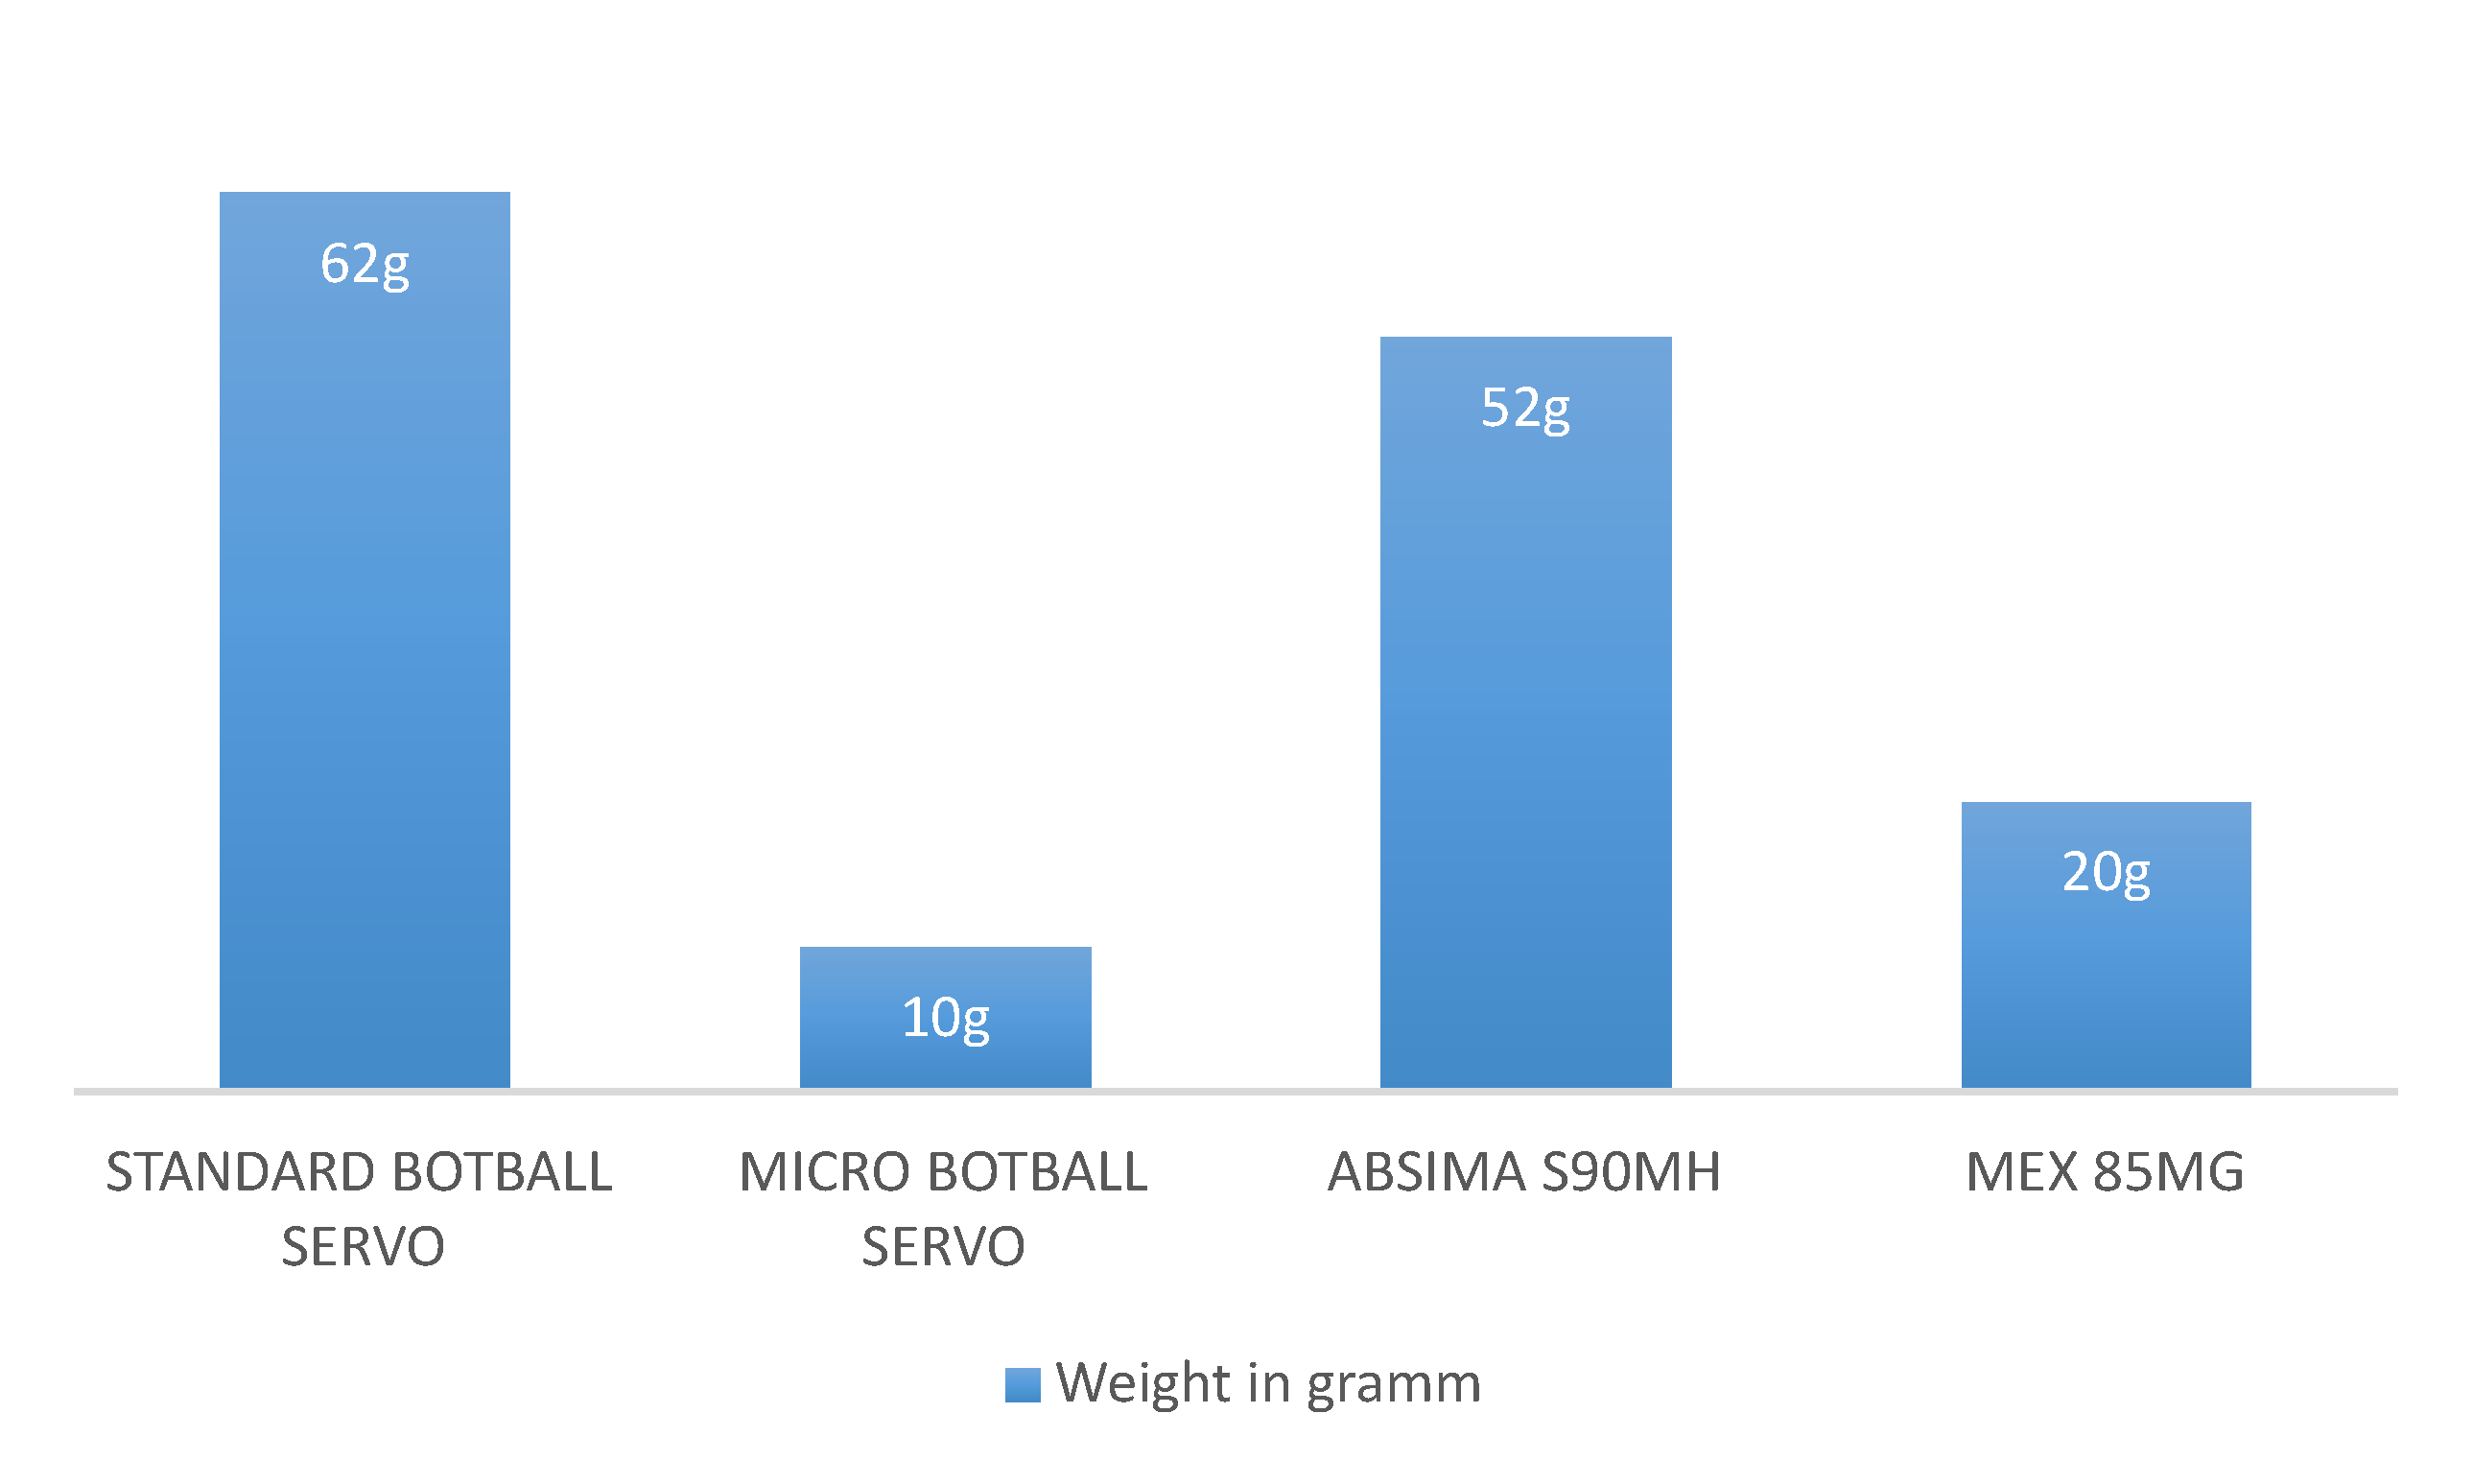
\includegraphics[width=0.50\textwidth,keepaspectratio]{weight_chart.pdf}
            \caption{Comparison of servo weight in gramm}
        \end{figure}

       As expected, there is a correlation between the size and weight of the servos in this case. The micro Botball servo, being smaller, is also lighter than its counterparts. Conversely, the standard Botball servo, being the largest, is the heaviest. It is important to note the different rotating mechanisms of the micro Botball servo compared to others, which must be taken into consideration when applying it. Thus, selecting the appropriate servo goes beyond just considering its size and weight. Designers must carefully evaluate how each servo's characteristics align with the specific requirements of their project.

    \subsection{Speed}
        In robotics, especially in competitive environments, servo speed is crucial. Servos must execute movements quickly to ensure optimal performance in competitions. The average of these measurements is presented in Figure 4.

        \begin{figure}[htbp]
            \centering
            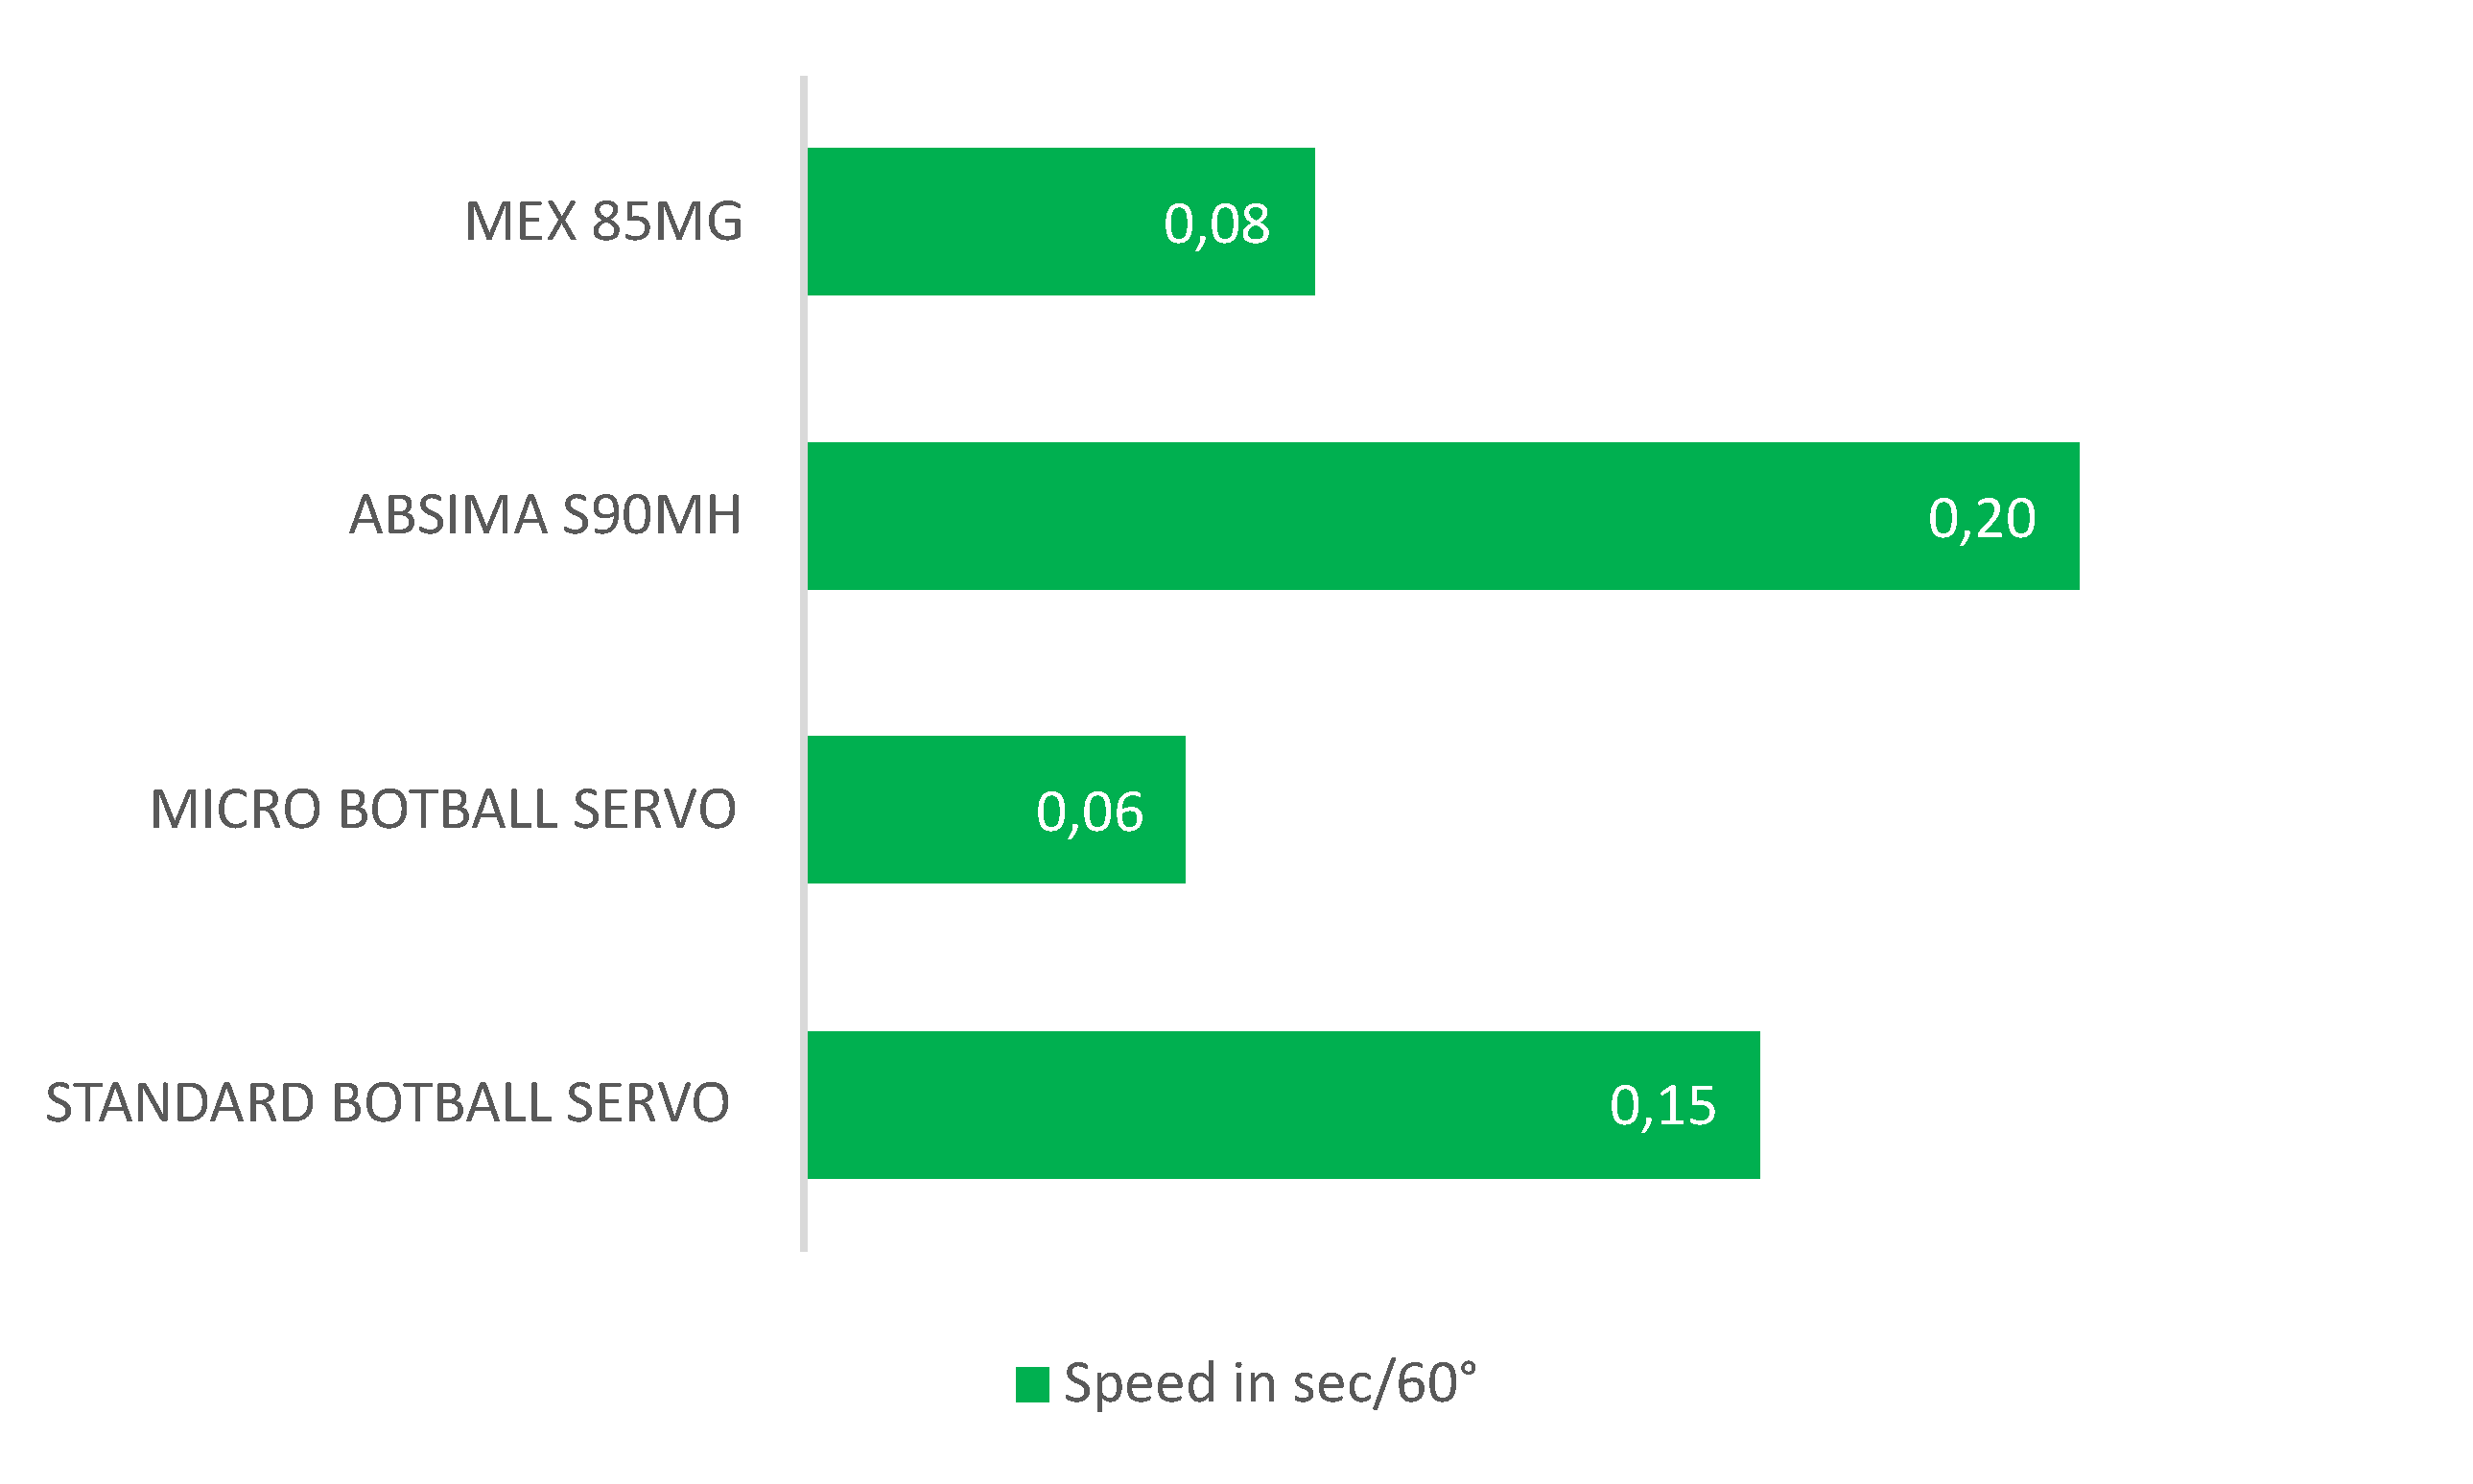
\includegraphics[width=0.50\textwidth,keepaspectratio]{speed_chart.pdf}
            \caption{Comparison of servo speed in sec/60°}
        \end{figure}

        Based on these findings, the micro Botball servo has the quickest response time, completing a 60-degree rotation in just 0.06 seconds. It is important to carefully select the servo to meet specific performance criteria, as even slight speed differentials can be decisive in competitive robotics.

    \subsection{Lifting Force}
        The lifting capacity of a servo is crucial when constructing any lifting mechanism, which is a necessity for every Botball tournament. The weight that a servo can lift determines whether it will break during testing or, even worse, during a tournament.

        \begin{figure}[htbp]
            \centering
            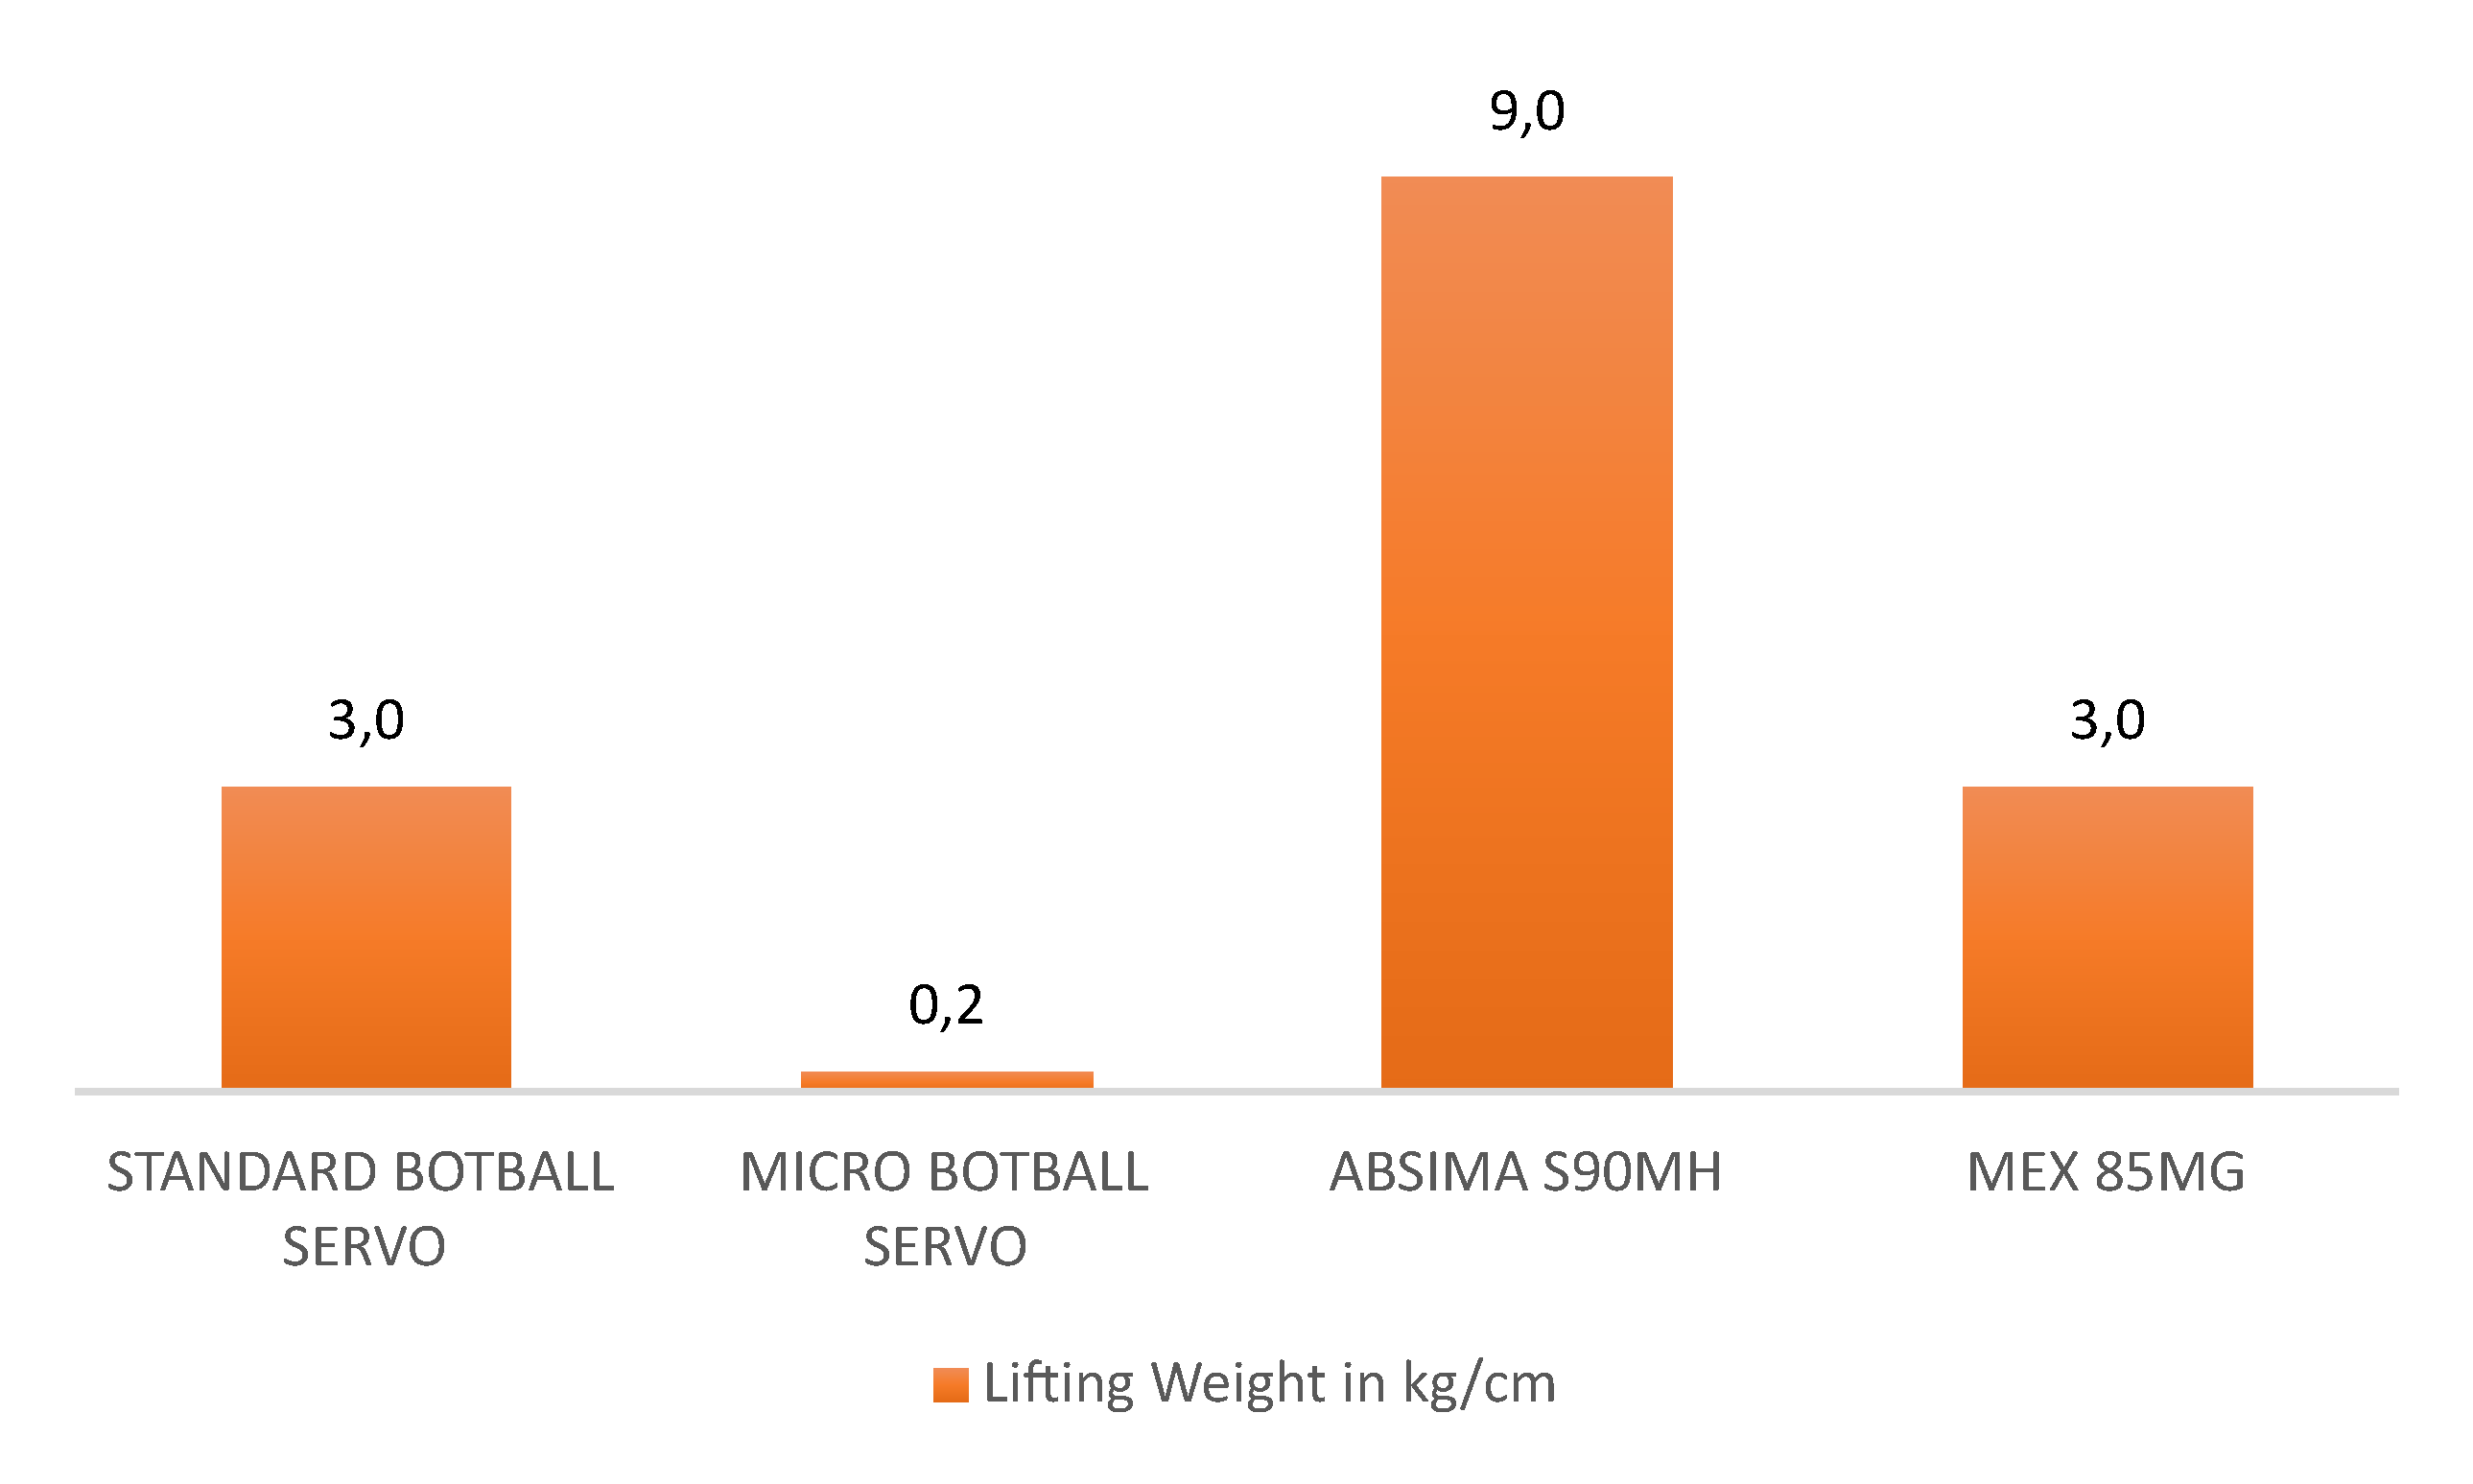
\includegraphics[width=0.50\textwidth,keepaspectratio]{lift_chart.pdf}
            \caption{Comparison of servo lifting weight}
        \end{figure}

        Figure 5 shows that the Absima S90MH and the MEX 85MG perform well in this category, while the Botball ones appear to be less impressive.   However, the Botball ones are sufficient for controlling a basic mechanism used in the Botball and OPEN tournaments. For heavier and more advanced mechanisms, we recommend using the Absima S90MH or MEX 85MG.

\section{Conclusion}
    The selection of a servo should be based on its intended application. This study provides valuable insights for tournament participants and hobbyists, helping them choose the most suitable servo for their unique circumstances.  
        
    The information provided includes standard Botball servos and potential alternatives. Stakeholders must now decide which servo is appropriate for their intended build.
        
    The Absima S90MH is recommended for tasks that require substantial lifting power, as it outperforms the standard Botball servo in capacity, albeit at the expense of reduced speed. Its compact size and lower weight make it an attractive alternative, provided the cost is justified. It is important to note that this recommendation is based solely on technical specifications and does not take into account any subjective evaluations.
        
    Conversely, the micro Botball servo is ideal for tasks that require high speed and low weight. It is worth noting that the MEX 85MG is marginally larger than the micro Botball servo, but surpasses it in velocity.  The micro Botball servo is recommended for designs prioritising speed over lifting capability, while the MEX 85MG should be considered when great force and speed are required at a good price.

\begin{thebibliography}{00}
    \bibitem{b1} Basics about servos\\
    \url{https://www.sparkfun.com/servos}\\
    \textsubscript{(last accessed on February 27, 2024)}\\
    
    \bibitem{b2} Servo database\\
    \url{https://servodatabase.com/servos/all} \\
    \textsubscript{(last accessed on February 27, 2024)}\\
    
    \bibitem{b3} Standard Botball servo\\
    \url{https://botball-swag.myshopify.com/collections/motos-and-servos/products/standard-servo} \\
    \textsubscript{(last accessed on February 27, 2024)}\\
    
    \bibitem{b4} Micro Botball servo\\
    \url{https://botball-swag.myshopify.com/collections/motos-and-servos/products/micro-servo} \\
    \textsubscript{(last accessed on February 27, 2024)}\\
    
    \bibitem{b5} MEX 85Mg servo\\
    \url{https://modster.at/komponenten-zubehoer/servos/2263/servo-mex-85mg-modster?c=170} \\
    \textsubscript{(last accessed on February 27, 2024)}\\
    
    \bibitem{b6} Absima S90MH servo\\
    \url{https://www.absima.shop/pp/absima-S90MH-9kg-servo-25t-metal-gear.htm?shop=absima_en&SessionId=&a=article&ProdNr=2030004&t=19114&c=19129&p=19129} \\
    \textsubscript{(last accessed on February 27, 2024)}\\
    
    \bibitem{b7} EUR/USD Exchange Rate\\
    \url{https://www.google.com/finance/quote/EUR-USD} \\
    \textsubscript{(last accessed on February 27, 2024)}\\
\end{thebibliography}
\end{document}